\documentclass[11pt]{article}

% ----- Packages -----
\usepackage{graphicx}
\usepackage{tikz}
\usetikzlibrary{positioning, arrows.meta, fit}
\usepackage{caption}
\usepackage{booktabs}
\usepackage{array}
\usepackage{geometry}
\usepackage{fancyhdr}
\usepackage{setspace}
\usepackage{titlesec}
\usepackage{float}
\usepackage{amsmath}
\usepackage{amssymb}
\usepackage{siunitx}        % consistent units + uncertainty typesetting
\usepackage{listings}
\usepackage{xcolor}
\usepackage{multirow}
\usepackage{placeins}
\usepackage{hyperref}
\hypersetup{
    colorlinks=true,
    urlcolor=blue,
    linkcolor=black,
    citecolor=black
}

% ----- Page Formatting -----
\geometry{margin=0.75in, columnsep=0.25in}
\setstretch{1.05}
\setlength{\emergencystretch}{3em}
\setlength{\parskip}{0.45em}
\setlength{\parindent}{0pt}
\setlength{\headheight}{13.6pt}

\titleformat{\section}{\normalfont\large\bfseries}{\thesection}{0.5em}{}
\titleformat{\subsection}{\normalfont\normalsize\bfseries}{\thesubsection}{0.5em}{}
\captionsetup{font=small, labelfont=bf}

% ----- Code Formatting -----
\lstset{
    basicstyle=\footnotesize\ttfamily,
    breaklines=true, columns=fullflexible, frame=single,
    keepspaces=true, showstringspaces=false, tabsize=4, language=Python
}

% ----- Header/Footer -----
\pagestyle{fancy}
\fancyhf{}
\lhead{PHY F353L Brownian Motion}
\rhead{Matzke}
\cfoot{\thepage}

% ==========================
\begin{document}

% ----- Full-Width Title and Abstract -----
\twocolumn[
\begin{center}
    {\Large \textbf{Counting Molecules by Watching Them Jostle:\\
    Boltzmann's Constant and Avogadro's Number from the\\
    Brownian Motion of Micron-Scale Spheres}}\\
    {\large Jacob Matzke (jam28248)}\\
    {\small Due: XX/XX/2026}
\end{center}

\begin{abstract}
A particle suspended in a fluid is ceaselessly buffeted by the fluid's molecules,
executing a random walk whose statistics encode the thermal energy scale $k_B T$.
We measured Boltzmann's constant and Avogadro's number by tracking the
two-dimensional Brownian motion of \SI{1}{\micro\meter}-diameter polystyrene spheres
in water under an optical microscope, recording 500-frame videos at 30 frames per
second with a monochrome camera calibrated at \SI{0.139}{\micro\meter} per pixel. A Python pipeline built on the \texttt{trackpy} implementation of the
Crocker--Grier algorithm located and linked the beads into trajectories, from which
we formed the ensemble mean-squared displacement (MSD); the diffusion coefficient
$D$ follows from its slope through the Einstein relation, and Boltzmann's constant
from the Stokes--Einstein relation $D = k_B T/6\pi\eta r$. Because localization error
makes the recovered $D$ depend on how much of the MSD is fit, we set the fit window
by Michalet's variance-optimal criterion ($x = 2.48 \Rightarrow p_{\min}=6$ lags) and
cross-checked $D$ against the regression-free covariance-based estimator (CVE). The
CVE disagreed by \SI{23}{\percent}; a sub-pixel-remainder diagnostic traced this to
detector pixel-locking, so we report it as a flagged upper bound. Our three
independent estimators bracket the accepted diffusion coefficient, and the primary
result is
$k_B = (1.54 \pm 0.15)\times10^{-23}~\si{\joule\per\kelvin}$ and
$N_A = (5.4 \pm 0.5)\times10^{23}~\si{\per\mole}$, both consistent with the accepted
values to within $\sim$$1.2\sigma$. The measurement is limited not by counting
statistics but by the systematic dependence of $D$ on the choice of
estimator---dominated by pixel-locking and a fast-bead selection bias---together with
the bead-size tolerance; we itemize each explicitly. The agreement confirms the
Einstein--Smoluchowski account of Brownian motion, by which a visible random walk is
made to weigh the molecules that drive it.
\end{abstract}

\vspace{1em}
]

% ==========================
\section{Introduction}
\label{Introduction}
In 1827 the botanist Robert Brown, watching pollen grains suspended in water through
a microscope, saw them jitter incessantly in a motion that never stopped and that he
could trace to no living agency. The explanation waited nearly eighty years: in 1905
Einstein, and independently Smoluchowski in 1906, showed that the jitter is the
visible accumulation of countless molecular impacts, and that its statistics are
quantitatively fixed by the thermal energy $k_B T$~\cite{einstein1905}. Einstein's
central result was that the mean-squared displacement of a suspended particle grows
linearly with time, with a coefficient---the diffusion constant---set by the
temperature, the fluid's viscosity, and the particle's size. This turned a
qualitative curiosity into a measuring instrument: by watching a particle diffuse,
one can count molecules. Jean Perrin did exactly that between 1908 and 1913,
extracting Avogadro's number from the motion of resin grains and, in doing so,
convincing the last skeptics that atoms are real---work for which he received the
1926 Nobel Prize in Physics~\cite{perrin1909}.

This experiment reproduces that determination with modern tools. We record the
Brownian motion of micron-scale polystyrene spheres in water with a digital
microscope, track their trajectories frame by frame, and form the mean-squared
displacement to extract the diffusion coefficient $D$. Inverting the Stokes--Einstein
relation with the known temperature, water viscosity, and bead size then yields
Boltzmann's constant $k_B$ and, through the gas constant, Avogadro's number $N_A$.
Because the diffusion coefficient is the only quantity we measure---everything else
is a tabulated constant or a calibration---the experiment is, at heart, the careful
determination of a single slope, and most of our effort goes into extracting that
slope without bias. We find
$k_B = (1.54\pm0.15)\times10^{-23}~\si{\joule\per\kelvin}$ and
$N_A = (5.4\pm0.5)\times10^{23}~\si{\per\mole}$, both consistent with the accepted
values to within $\sim$$1.2\sigma$, confirming the Einstein--Smoluchowski description
of Brownian motion.

\subsection{Theory}
\label{Theory}
A spherical particle suspended in a fluid feels two influences from the surrounding
molecules: a rapidly fluctuating random force that drives its motion, and a
systematic viscous drag that opposes it. Einstein and Smoluchowski showed that these
are two faces of the same molecular agitation, and that their balance fixes the
particle's diffusion.

\textbf{Random walk and the diffusion coefficient.} Over times long compared with the
molecular collision time, the particle performs a random walk. In the two dimensions
recorded by the camera, the ensemble-averaged mean-squared displacement grows
linearly with time~\cite{qian},
\begin{equation}
    \langle \Delta r^2(t)\rangle = 4 D t,
    \label{eq:randomwalk}
\end{equation}
where $D$ is the diffusion coefficient and the factor $4 = 2d$ with dimensionality
$d = 2$ (each Cartesian coordinate contributes $2Dt$).

\textbf{The Einstein relation.} Einstein connected $D$ to the thermal energy by
balancing diffusion against drag: a particle with drag coefficient $\gamma$ in
thermal equilibrium at temperature $T$ diffuses with
\begin{equation}
    D = \frac{k_B T}{\gamma},
    \label{eq:einstein}
\end{equation}
the fluctuation--dissipation relation for Brownian motion~\cite{reif}.

\textbf{Stokes drag and Stokes--Einstein.} For a sphere of radius $r$ moving slowly
through a fluid of dynamic viscosity $\eta$, the drag coefficient is given by Stokes'
law, $\gamma = 6\pi\eta r$. Substituting into Equation~\eqref{eq:einstein} gives the
Stokes--Einstein relation,
\begin{equation}
    D = \frac{k_B T}{6\pi\eta r}.
    \label{eq:se}
\end{equation}
Every quantity on the right except $k_B$ is known or measured---$T$ with a
thermometer, $\eta(T)$ from tabulated water data, and $r$ from the bead
specification---so a measurement of $D$ determines Boltzmann's constant, and through
the molar gas constant $R$, Avogadro's number:
\begin{equation}
    k_B = \frac{6\pi\,\eta(T)\,r\,D}{T},
    \qquad
    N_A = \frac{R}{k_B}.
    \label{eq:kbtheory}
\end{equation}

\textbf{Localization error.} A real measurement locates each particle only to a
finite precision $\sigma_{\text{loc}}$, which adds a constant term $4\sigma_{\text{loc}}^2$
to the ideal linear growth of Equation~\eqref{eq:randomwalk}; we treat this offset
explicitly in the analysis (Section~\ref{ssec:msd}). The closely related question of
how many lag times to include when fitting the slope is what makes the choice of
estimator, rather than counting statistics, the limiting consideration in this
experiment.

% ==========================
\section{Experimental Apparatus}
\label{Experimental Apparatus}
Our apparatus follows the standard configuration for this measurement~\cite{nakroshis},
sketched in Figure~\ref{fig:schematic}: a monochrome digital camera mounted on an
upright optical microscope, viewing micron-scale spheres in a water cell on the
stage, with the whole instrument resting on vibration-isolating pads. Brightfield
illumination passes up through the sample from below; a frosted, infrared-absorbing
glass in the illumination path removes heat that would otherwise drive convective
currents in the water and overwhelm the thermal motion we wish to measure.

\textbf{Microscope and camera.} The microscope was an Olympus compound microscope.
Images were captured by a ThorLabs scientific camera and recorded with the ThorCam
desktop application, which delivered 8-bit monochrome frames of $1024\times768$
pixels.

\textbf{Spatial calibration.} The pixel-to-length scale was fixed by imaging a
ThorLabs stage-micrometer calibration slide under identical optics: a
\SI{50}{\micro\meter} interval of its ruling spanned $360$ pixels, giving a
calibration of $\text{mpp} = 50/360 = \SI{0.139}{\micro\meter}$ per pixel and a field
of view of about $142\times107~\si{\micro\meter}$. Because the diffusion coefficient
scales as the \emph{square} of this length, the calibration uncertainty
($\pm\SI{0.002}{\micro\meter}$/px) enters the error budget doubled
(Section~\ref{ssec:budget}).

\textbf{Temperature.} The sample temperature sets the water viscosity $\eta(T)$ and
appears directly in the Stokes--Einstein inversion
(Equation~\eqref{eq:kbtheory}), so it must be measured rather than assumed. We
recorded it with a Kane--May workshop digital thermometer fitted with a probe,
reading \SI{25.9}{\celsius}.

\textbf{Acquisition.} Videos were recorded at 30 frames per second in
500-frame batches---500 frames being the largest single file the ThorCam TIFF export
produces---and saved directly as multi-page TIFF stacks with no in-software
processing. Each stack is one trial in the analysis (Section~\ref{Data}).

\textbf{Vibration isolation.} As in the reference configuration, the instrument
rested on Sorbothane pads to damp building and bench vibration, which would otherwise
add coherent, non-thermal displacements to the beads and bias the diffusion
measurement.

\begin{figure}[tb]
\centering
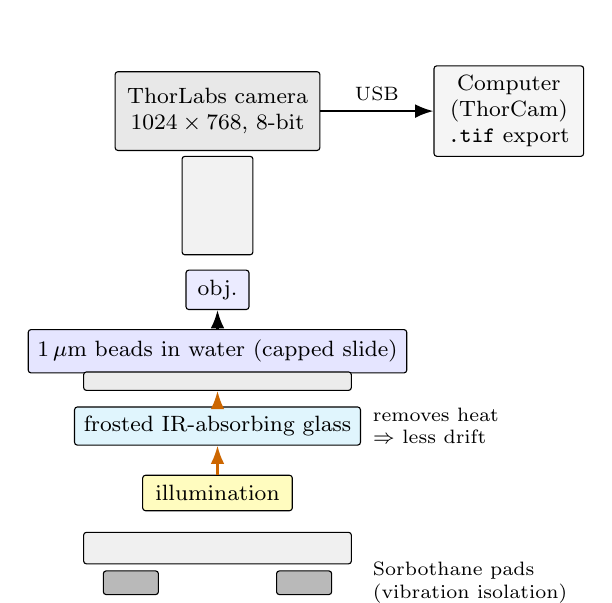
\begin{tikzpicture}[>=Latex, font=\footnotesize,
  box/.style={draw, align=center, rounded corners=1pt}]
  % --- stacked components (side view) ---
  \node[box, fill=gray!18, minimum width=2.6cm, minimum height=1.0cm] (cam) at (0,6.05)
       {ThorLabs camera\\$1024\times768$, 8-bit};
  \node[box, fill=gray!10, minimum width=0.9cm, minimum height=1.25cm] (body) at (0,4.85) {};
  \node[box, fill=blue!8, minimum width=0.8cm, minimum height=0.5cm] (obj) at (0,3.78) {obj.};
  \node[box, fill=blue!10, minimum width=3.0cm, minimum height=0.55cm] (samp) at (0,3.0)
       {1\,$\mu$m beads in water (capped slide)};
  \node[box, fill=gray!15, minimum width=3.4cm, minimum height=0.18cm] (stage) at (0,2.62) {};
  \node[box, fill=cyan!12, minimum width=2.6cm, minimum height=0.42cm] (ir) at (0,2.05)
       {frosted IR-absorbing glass};
  \node[box, fill=yellow!25, minimum width=1.9cm, minimum height=0.45cm] (lamp) at (0,1.2)
       {illumination};
  \node[box, fill=gray!12, minimum width=3.4cm, minimum height=0.4cm] (base) at (0,0.5) {};
  \node[box, fill=gray!55, minimum width=0.7cm, minimum height=0.3cm] at (-1.1,0.06) {};
  \node[box, fill=gray!55, minimum width=0.7cm, minimum height=0.3cm] at (1.1,0.06) {};
  % --- light path (illumination up through the sample) ---
  \draw[->, orange!80!black, thick] (lamp.north) -- (ir.south);
  \draw[->, orange!80!black, thick] (ir.north) -- (stage.south);
  \draw[->, thick] (samp.north) -- (obj.south);
  % --- computer ---
  \node[box, fill=gray!8, minimum width=1.9cm, minimum height=0.95cm] (pc) at (3.7,6.05)
       {Computer\\(ThorCam)\\\texttt{.tif} export};
  \draw[->, thick] (cam.east) -- node[above, font=\scriptsize]{USB} (pc.west);
  % --- side labels ---
  \node[right, font=\scriptsize, align=left] at (1.85,2.05) {removes heat\\$\Rightarrow$ less drift};
  \node[right, font=\scriptsize, align=left] at (1.85,0.06) {Sorbothane pads\\(vibration isolation)};
\end{tikzpicture}
\caption{Schematic of the microscope setup (side view), in the standard configuration
for this measurement~\cite{nakroshis}. Brightfield light passes up from the
illumination through a frosted, infrared-absorbing glass and the capped water cell,
into the objective, and up the microscope body to a ThorLabs monochrome camera; the
digitized $1024\times768$ frames are read out over USB by ThorCam and saved as TIFF
stacks. Sorbothane pads under the base isolate the instrument from vibration.}
\label{fig:schematic}
\end{figure}

% ==========================
\FloatBarrier
\section{Experimental Procedure}
\label{Experimental Procedure}
We followed the same basic procedure for every trial, refining the sample
preparation as we learned what produced stable, drift-free imaging.

\textbf{Cleaning and first preparation.} All optical surfaces---slides, cover slips,
and the objective lens---were cleaned thoroughly before use, since dust and residue
both scatter light and seed convective currents. Our first preparation placed three
drops of the \SI{1}{\micro\meter}-diameter polystyrene-sphere suspension into the
well of a concave (depression) microscope slide, left open to the air. This proved
unsatisfactory: the open water surface drove a persistent bulk drift, and the imaging
was acutely sensitive to how level the stage was and to air currents from the room's
air conditioning, so the beads' motion was dominated by flow rather than diffusion
and the results were unreliable.

\textbf{Capped preparation.} We therefore switched to a capped cell: two drops of the
suspension in the depression slide, covered with a slip whose excess fluid was wiped
away. Capping the cell suppressed the evaporation- and air-driven currents and gave
markedly more stable, repeatable bead motion; this is the configuration used for all
reported trials, and the origin of the ``capped'' label on the data.

\textbf{Settling and acquisition.} Recording trials over roughly forty minutes, we
observed that both the number of beads in the focal plane and the steadiness of their
imaging improved with time. We attribute this to the beads settling toward a common
equilibrium depth, so that progressively more of them lie within the microscope's
shallow depth of focus---the same settling behavior noted by Nakroshis
\textit{et~al.}~\cite{nakroshis}. We accordingly drew our best data from the later
trials. Each trial was a 500-frame video recorded at 30 frames per second in ThorCam
and exported directly as a TIFF stack (Section~\ref{Data}); the analyzed
best-controlled trial additionally had its small residual drift removed in software
(Section~\ref{ssec:drift}).

% ==========================
\FloatBarrier
\section{Data}
\label{Data}
Each trial is stored as a single multi-page TIFF stack exactly as exported by
ThorCam: 500 frames of $1024\times768$ 8-bit monochrome pixels, recorded at 30 frames
per second, with no in-software smoothing or background subtraction applied. At the
calibrated scale of \SI{0.139}{\micro\meter}/px this is a field of view of roughly
$142\times107~\si{\micro\meter}$. Because the camera writes the frames directly,
essentially no preprocessing or format conversion was needed before analysis; the
pipeline of Section~\ref{Analysis} reads the TIFF stack as recorded. The water
temperature, which sets the viscosity in the Stokes--Einstein inversion, was
\SI{25.9}{\celsius}.

Figure~\ref{fig:raw} shows a representative raw frame. The microspheres appear as
small, round, low-contrast spots that are \emph{darker} than the background, each
surrounded by a brighter diffraction halo because the bead sits slightly out of the
focal plane (panel~b). Two features visible here set the agenda for the analysis: the
beads are low-contrast against a noticeably noisy background, so a simple brightness
threshold is a poor locator and we instead band-pass filter and centroid each bead
(Section~\ref{ssec:detect}); and each bead moves only a fraction of its diameter
between successive frames, which sets the per-frame search radius used to link
detections into trajectories (Section~\ref{ssec:link}).

\begin{figure}[tb]
    \centering
    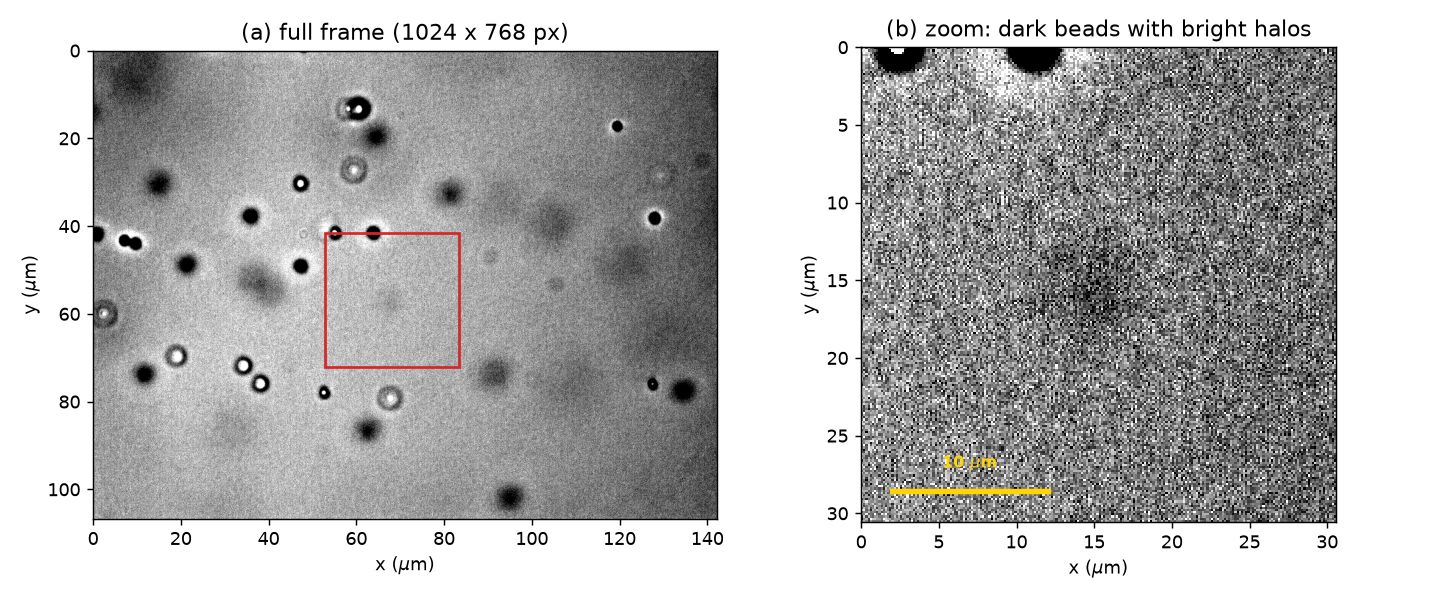
\includegraphics[width=\linewidth]{Images/D2T7_raw_frame.png}
    \caption{Representative raw frame (best-controlled trial), contrast-stretched for
    display. (a)~The full $1024\times768$ field of view ($\sim$$142\times107~\si{\micro
    \meter}$); the dark microspheres are scattered across a flat background. (b)~A
    zoom (red box) showing the low-contrast dark beads, their bright diffraction
    halos, and the point-to-point image noise. Axes are in microns from the
    calibration; the scale bar in (b) is \SI{10}{\micro\meter}.}
    \label{fig:raw}
\end{figure}

% ==========================
\FloatBarrier
\section{Analysis}
\label{Analysis}
We developed a Python pipeline to turn the recorded videos into a diffusion
coefficient and, through the Stokes--Einstein relation, into Boltzmann's constant
and Avogadro's number, following the established video-microscopy approach to this
measurement~\cite{nakroshis}; the full code is available on GitHub (Appendix~A). The
pipeline (i)~locates every bead in every frame, (ii)~links those detections into
trajectories, (iii)~removes residual drift, (iv)~builds the ensemble mean-squared
displacement (MSD) and extracts $D$ with a localization-error-aware fit, and
(v)~inverts Stokes--Einstein with full uncertainty propagation. Because the
extracted $D$ turns out to depend on the choice of estimator, we deliberately
compute it three independent ways and carry the spread as a systematic. We present
our best-controlled trial---a capped sample cell with residual drift removed---as
the worked example; the same pipeline applies unchanged to the other recorded
trials.

\subsection{Detecting the microspheres}
\label{ssec:detect}
The beads appear as small, round, low-contrast objects that are \emph{darker} than
the background, each ringed by a brighter diffraction halo (the bead sits slightly
out of the focal plane). We locate them with \texttt{trackpy}'s implementation of
the Crocker--Grier centroid algorithm~\cite{crockergrier,trackpy}: each frame is
band-pass filtered to suppress pixel noise and the slowly varying, uneven
illumination, local intensity extrema are found, and each candidate is refined to a
sub-pixel centroid by its brightness-weighted center of mass. Because the beads are
darker than the background we run the finder on the inverted image; a minimum
integrated-brightness threshold (\texttt{minmass}) rejects noise peaks. We verified
explicitly that the bright halos are the diffraction rings of the \emph{same}
particles rather than separate objects (their detections are weak and sit a bead
radius off each dark core), so detecting only the dark cores counts each bead
exactly once. A representative frame with the recovered trajectories overlaid is
shown in Figure~\ref{fig:tracks}.

\begin{figure}[tb]
    \centering
    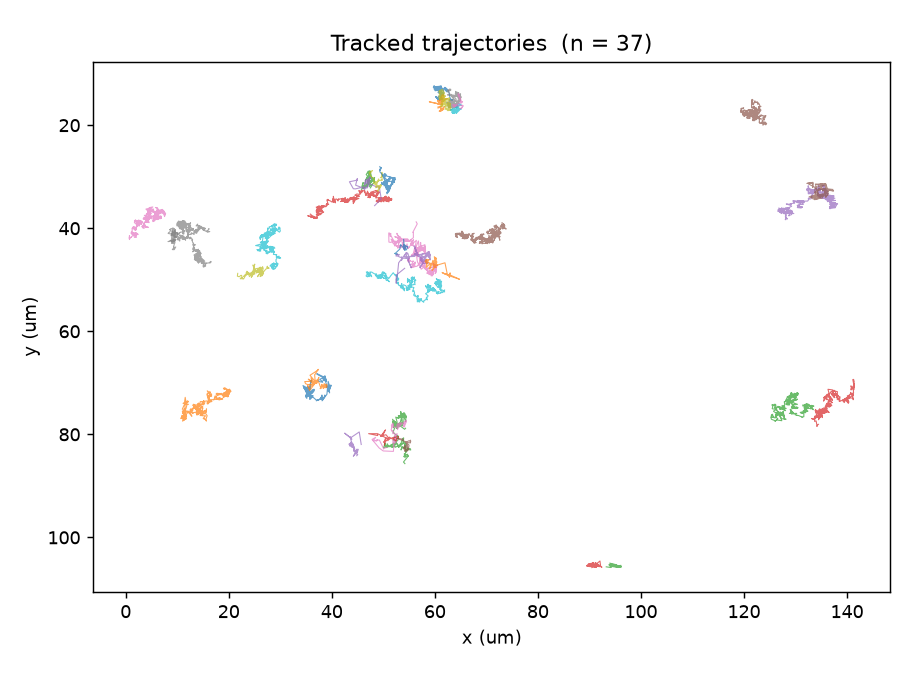
\includegraphics[width=\linewidth]{Images/D2T7_Capped_tracks.png}
    \caption{Recovered bead trajectories overlaid on the field of view. Each
    coloured track is one microsphere followed across frames; the random,
    space-filling paths are the visual signature of Brownian motion.}
    \label{fig:tracks}
\end{figure}

\subsection{Linking detections into trajectories}
\label{ssec:link}
Detections in successive frames are linked into trajectories by nearest-neighbour
assignment within a maximum per-frame search radius, with a short \emph{memory} that
bridges momentary detection dropouts so a bead is not given a new identity when it
briefly fades~\cite{trackpy}. Crucially we use \emph{no} velocity predictor: because
Brownian displacements are random and uncorrelated, predicting the next position
from the previous step actively mis-guides the linker and fragments tracks (we
confirmed this empirically---adding a predictor collapsed the usable track count).
Trajectories shorter than a minimum length are discarded as spurious
(\texttt{filter\_stubs}), since a real bead persists for many frames while noise
flickers in and out. This yields $N \approx 37$ well-sampled trajectories with a
median length of $\sim$140 frames.

\subsection{Removing residual drift}
\label{ssec:drift}
Although the cell was capped to suppress evaporation-driven flow, a small coherent
drift of the whole bead population remains. Because drift adds a \emph{directed}
component to every displacement, it inflates the MSD and hence $D$. We estimate the
drift as the ensemble-mean displacement per frame and subtract it before the MSD
analysis, so that only the random thermal component survives. For this trial the
subtraction lowered $D$ by $\sim$9\%, confirming a real but modest flow.

\subsection{The mean-squared displacement and \texorpdfstring{$D$}{D}}
\label{ssec:msd}
For two-dimensional Brownian motion the ensemble MSD grows linearly with lag
time~$t$~\cite{einstein1905,qian},
\begin{equation}
    \langle \Delta r^2(t)\rangle = 4 D t + 4\sigma_{\text{loc}}^2 ,
    \label{eq:msd}
\end{equation}
where the constant offset $4\sigma_{\text{loc}}^2$ is the \emph{static localization
error}---the finite precision with which each centroid is measured, which displaces
the MSD upward by a fixed amount at all lags. Fitting a straight line to the
short-lag MSD gives $D$ from the slope and $\sigma_{\text{loc}}\approx\SI{200}{\nano
\meter}$ from the intercept (Figure~\ref{fig:msd}). The MSD is visibly linear
($R^2 = 0.999$). We also report the anomalous-diffusion exponent $\alpha$
(defined by $\langle\Delta r^2\rangle\sim t^{\alpha}$): a naive power-law fit to the
raw MSD is biased low by the offset, but once the offset is removed
$\alpha = 0.96$, consistent with ordinary, non-anomalous Brownian diffusion.

\begin{figure}[tb]
    \centering
    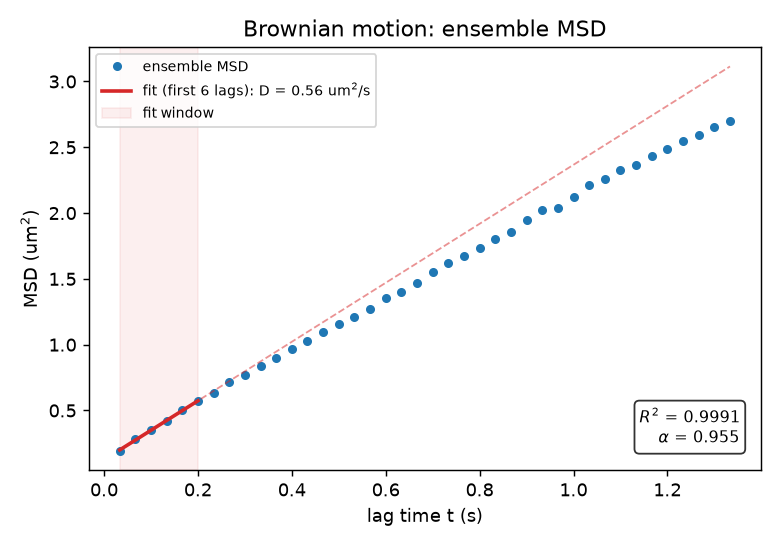
\includegraphics[width=\linewidth]{Images/D2T7_Capped_msd.png}
    \caption{Ensemble MSD versus lag time. The short-lag linear fit (red) gives
    $D$ from its slope via Equation~\eqref{eq:msd}; the small positive intercept is
    the localization-error floor. The curve is linear over the fitted window
    ($R^2 = 0.999$), the hallmark of ordinary diffusion.}
    \label{fig:msd}
\end{figure}

\subsection{Choosing the fit window: localization error and Michalet's optimum}
\label{ssec:michalet}
Localization error makes the MSD curve subtly away from a perfect straight line, so
the fitted slope---and hence $D$---depends on \emph{how many} lags are included.
Michalet~\cite{michalet2010} showed that the variance of the MSD-derived $D$ is
minimized at a specific number of points set by the dimensionless \emph{reduced
localization error}
\begin{equation}
    x = \frac{\sigma_{\text{loc}}^2}{D\,\Delta t},
    \qquad
    p_{\min} = \big\lfloor 2 + 2.7\sqrt{x}\,\big\rfloor ,
    \label{eq:michalet}
\end{equation}
where $\Delta t$ is the frame interval (Michalet 2010, Eqs.~20 and~30). From our fit
$x = 2.48$, giving $p_{\min} = 6$ lags, which we adopt as the \emph{primary} fit
window. Fitting more lags is not harmless: the recovered $D$ drifts steadily
downward as longer lags are added (Figure~\ref{fig:fitwindow}a), because faster
beads diffuse out of the field of view sooner and the long-lag MSD is increasingly
dominated by the slower survivors---a \emph{selection bias} rather than true
sub-diffusion. We carry the spread of $D$ across fit windows (from $p_{\min}$ to a
naive long window) as a fit-window systematic of $\pm 5.9\%$.

\begin{figure*}[tb]
    \centering
    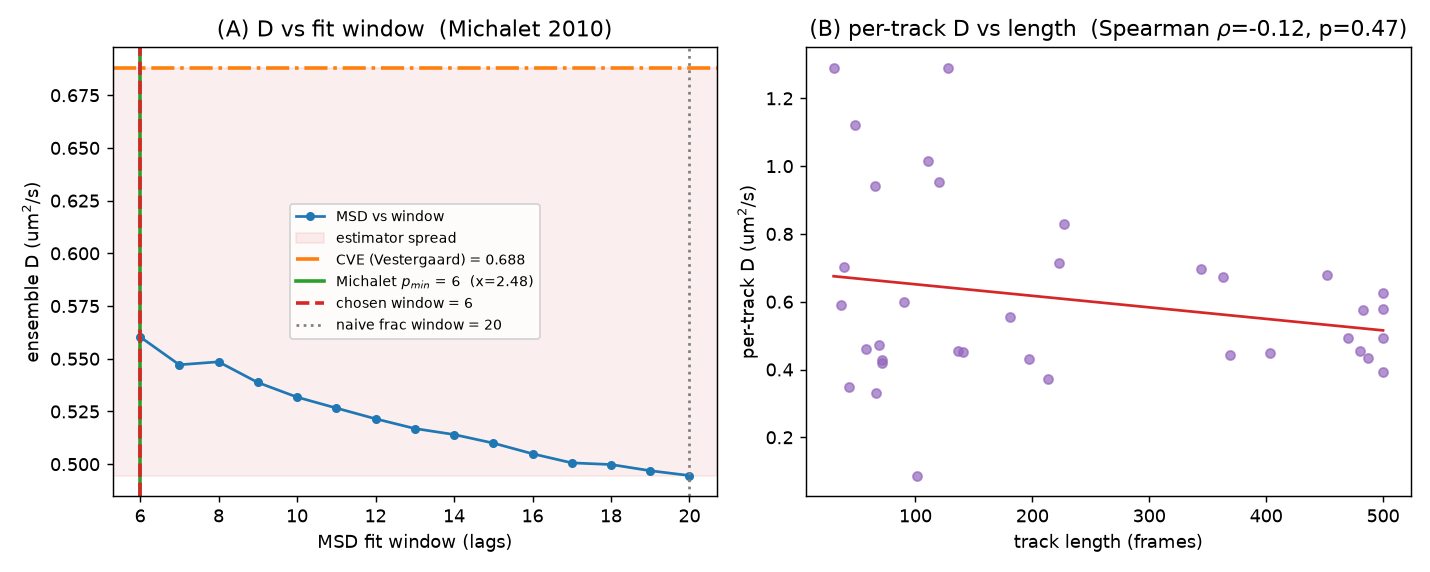
\includegraphics[width=\linewidth]{Images/D2T7_Capped_fitwindow.png}
    \caption{(a)~Diffusion coefficient versus MSD fit window. $D$ drifts downward as
    longer lags enter (fast-bead selection bias); the Michalet optimum $p_{\min}=6$
    (green) is adopted, and the CVE estimator (orange) is overlaid. The shaded band
    is the estimator spread. (b)~Per-track $D$ versus track length: after rejecting
    one outlier bead the residual length--$D$ correlation is weak, but panel~(a)
    establishes the window dependence directly.}
    \label{fig:fitwindow}
\end{figure*}

\subsection{An independent estimator and a localization diagnostic}
\label{ssec:cve}
To check the MSD result without fitting an MSD at all, we also computed the
covariance-based estimator (CVE) of Vestergaard
\textit{et~al.}~\cite{vestergaard},
\begin{equation}
    \hat{D}_{\text{CVE}} = \frac{\langle \Delta x_n^2\rangle}{2\Delta t}
    + \frac{\langle \Delta x_n\,\Delta x_{n+1}\rangle}{\Delta t},
    \label{eq:cve}
\end{equation}
in which the negative lag-1 covariance term exactly cancels the localization-error
and motion-blur inflation, making $\hat D$ unbiased \emph{without} fitting. The CVE
returns $D_{\text{CVE}} = \SI{0.688}{\micro\meter\squared\per\second}$, fully
$+23\%$ above the MSD value. Rather than average this in, we asked \emph{why} it
disagrees. The CVE assumes the localization error is white (uncorrelated frame to
frame); we tested that assumption with the sub-pixel-remainder histogram
(Figure~\ref{fig:subpixel}), the standard pixel-locking check (built into
\texttt{trackpy} as \texttt{subpx\_bias}). The remainders are strongly non-uniform,
piling up at integer-pixel positions (modulation $67\%$ in $x$, $121\%$ in $y$):
the localization is \emph{pixel-locked}, so its error is correlated, not white. This
is exactly the regime in which the CVE is known to be biased~\cite{berglund,
michaletberglund,savindoyle}. We therefore report $D_{\text{CVE}}$ for transparency
but flag it as a (high) upper bound and exclude it from the systematic.

\begin{figure}[tb]
    \centering
    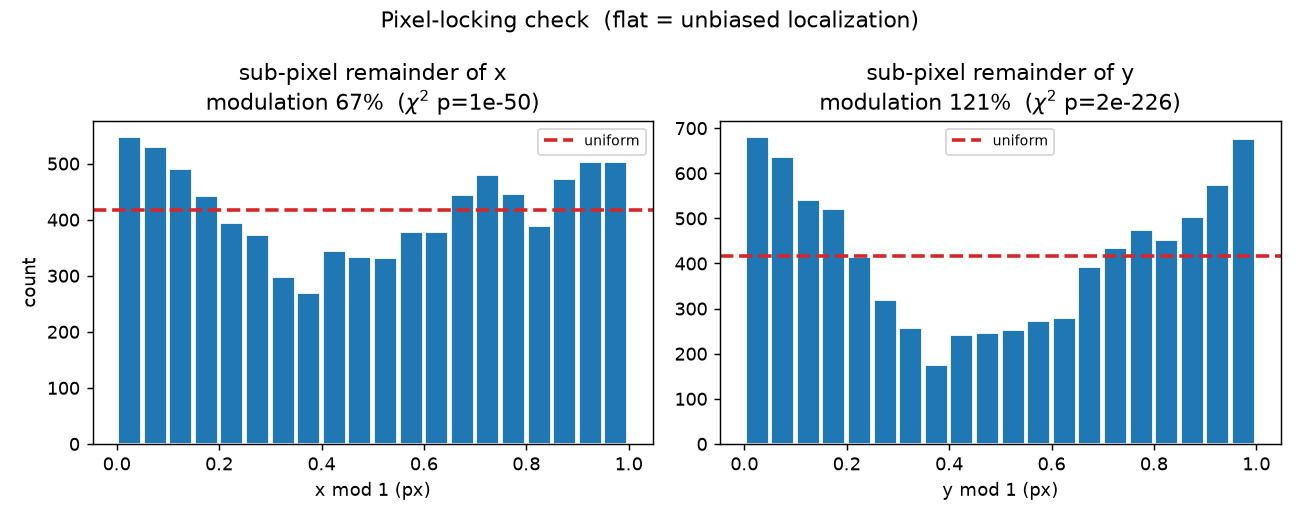
\includegraphics[width=\linewidth]{Images/D2T7_Capped_subpixel_bias.png}
    \caption{Pixel-locking check: histogram of the sub-pixel remainder of the bead
    positions ($x,y \bmod 1$~px). Unbiased localization would be uniform (dashed);
    the strong pile-up at integer pixels (modulation $67\%$/$121\%$) shows the
    centroids are locked to the pixel grid, so the localization error is correlated.
    This is why the CVE (Equation~\eqref{eq:cve}) is treated as an upper bound.}
    \label{fig:subpixel}
\end{figure}

\subsection{Three estimators and the method systematic}
\label{ssec:three}
For scientific integrity we report $D$ from all three independent estimators rather
than a single number (Table~\ref{tab:estimators}). The accepted free-diffusion value
implied by the literature $k_B$, $D_{\text{theory}} =
\SI{0.502}{\micro\meter\squared\per\second}$, lies \emph{inside} this range. We adopt
the Michalet-optimal MSD value as primary and define the method (fit-window)
systematic as the half-range of the MSD estimators, $\pm 5.9\%$; the pixel-locking
diagnostic justifies leaving the CVE out of that spread.

\begin{table}[h]
    \centering
    \footnotesize
    \setlength{\tabcolsep}{4pt}
    \begin{tabular}{@{}lcl@{}}
        \toprule
        Estimator & $D$ (\si{\micro\meter\squared\per\second}) & Note \\
        \midrule
        CVE (Vestergaard)        & $0.688$ & upper bound (pixel-locking) \\
        MSD @ $p_{\min}=6$        & $0.560$ & \textbf{primary} (Michalet) \\
        MSD @ long window         & $0.495$ & selection-bias floor \\
        \midrule
        \textit{literature $D$}   & $0.502$ & lies within the range \\
        \bottomrule
    \end{tabular}
    \caption{Three independent estimates of $D$ bracket the literature value. The
    Michalet-optimal MSD value is adopted as primary; the CVE is a flagged upper
    bound (Section~\ref{ssec:cve}).}
    \label{tab:estimators}
\end{table}

\subsection{Robustness: outlier rejection, bootstrap, and step statistics}
\label{ssec:robust}
Three checks guard the central value and its statistical error. First, a handful of
trajectories are mis-linked or atypical; we reject per-bead $D$ outliers beyond
$3.5$ median-absolute-deviations from the median (one bead removed here), which also
de-inflates the per-bead mean. Second, because $k_B$ uses the \emph{ensemble} $D$,
we quote its statistical error from a bead-level \emph{bootstrap}---resampling whole
trajectories with replacement and recomputing the ensemble $D$---rather than the
per-bead standard error of the mean, which mismatches the estimator and is overly
conservative; the bootstrap gives $D_{\text{stat}} = 5.0\%$. Third, the
distribution of single-frame displacements is Gaussian
(Figure~\ref{fig:displacements}), as Equation~\eqref{eq:msd} requires for genuine
diffusion; the slight excess peakedness is consistent with the bead-to-bead spread
in $D$.

\begin{figure}[tb]
    \centering
    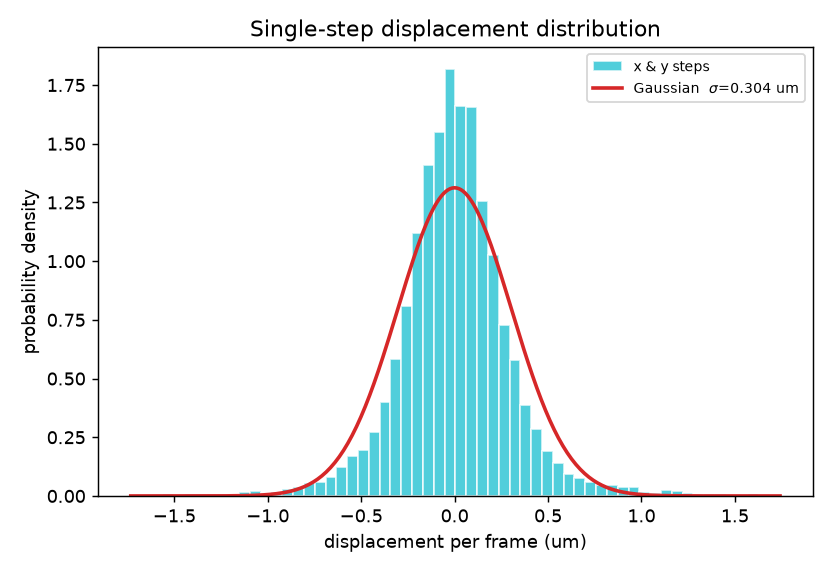
\includegraphics[width=\linewidth]{Images/D2T7_Capped_displacements.png}
    \caption{Distribution of single-frame step displacements (pooled over $x$, $y$,
    and all beads) with a zero-mean Gaussian overlay. The Gaussian form is the
    expected signature of Brownian motion. The $y$-axis is a probability
    \emph{density} (units \si{\per\micro\meter}), so values exceeding $1$ are normal
    for a sub-micron-wide distribution.}
    \label{fig:displacements}
\end{figure}

\subsection{From \texorpdfstring{$D$}{D} to Boltzmann's constant and \texorpdfstring{$N_A$}{NA}}
\label{ssec:stokes}
A sphere of radius $r$ diffusing in a fluid of viscosity $\eta$ at temperature $T$
obeys the Stokes--Einstein relation $D = k_B T/(6\pi\eta r)$, so
\begin{equation}
    k_B = \frac{6\pi\,\eta(T)\,r\,D}{T},
    \qquad
    N_A = \frac{R}{k_B},
    \label{eq:kb}
\end{equation}
with $R$ the molar gas constant. Using the bead radius $r = \SI{0.5}{\micro\meter}$,
the measured temperature $T = \SI{299.05}{\kelvin}$ ($\SI{25.9}{\celsius}$), and the
tabulated viscosity of water at that temperature, $\eta = \SI{8.72e-4}{\pascal\second}$,
the primary $D$ gives
\begin{equation}
\begin{aligned}
    k_B &= (1.54 \pm 0.15)\times10^{-23}~\si{\joule\per\kelvin},\\
    N_A &= (5.4 \pm 0.5)\times10^{23}~\si{\per\mole}.
\end{aligned}
\end{equation}
The spatial calibration enters here: positions are converted from pixels to microns
with $\text{mpp} = 50/360 = \SI{0.139}{\micro\meter}$/px, and because $D$ scales as
the \emph{square} of this length, its fractional error doubles in the budget below.

\subsection{Uncertainty budget}
\label{ssec:budget}
We tracked each source separately and combined them in quadrature
(Table~\ref{tab:budget}). The budget is notably \emph{balanced}: no single term
dominates. The fit-window/estimator systematic ($5.9\%$, Section~\ref{ssec:three}),
the bead-radius tolerance ($5.0\%$, from the $\pm\SI{0.05}{\micro\meter}$ size
specification, propagated as $\sigma_r/r$), and the bootstrap statistical error
($5.0\%$) are all comparable; the calibration term is $2\sigma_{\text{mpp}}/
\text{mpp} = 2.9\%$ (the factor of two because $D\propto\text{mpp}^2$); and the
temperature term is negligible. Combined,
\begin{equation}
    \frac{\delta k_B}{k_B} = 9.6\%
    \;\Longrightarrow\;
    k_B = (1.54\pm0.15)\times10^{-23}~\si{\joule\per\kelvin}.
\end{equation}

\begin{table}[h]
    \centering
    \footnotesize
    \setlength{\tabcolsep}{4pt}
    \begin{tabular}{@{}lcc@{}}
        \toprule
        Source & Rel.\ contribution & Type \\
        \midrule
        $D$ method / fit window      & $5.9\%$ & syst. \\
        Bead radius ($\pm0.05~\si{\micro\meter}$) & $5.0\%$ & syst. \\
        $D$ statistical (bootstrap)  & $5.0\%$ & random \\
        Calibration ($2\,\sigma_{\text{mpp}}$) & $2.9\%$ & syst. \\
        Temperature                  & $0.1\%$ & syst. \\
        \midrule
        Total (quadrature)           & $9.6\%$ & \\
        \bottomrule
    \end{tabular}
    \caption{Relative uncertainty budget for $k_B$ (and $N_A$, which inherits the
    same fractional error). The CVE is excluded from the $D$-method term because the
    pixel-locking diagnostic (Section~\ref{ssec:cve}) shows it is biased.}
    \label{tab:budget}
\end{table}

% ==========================
\FloatBarrier
\section{Discussion}
\label{Discussion}
The experiment set out to convert the visible jitter of micron-scale spheres into a
measurement of Boltzmann's constant and Avogadro's number. This section compares the
result with the accepted values, interprets it physically, and examines the
estimator dependence and the dominant uncertainties.

\subsection{Comparison with accepted values}
\label{ssec:comparison}
Table~\ref{tab:comparison} compares our results with the accepted constants. The
primary diffusion coefficient, $D = \SI{0.560}{\micro\meter\squared\per\second}$,
yields $k_B = (1.54\pm0.15)\times10^{-23}~\si{\joule\per\kelvin}$ and
$N_A = (5.4\pm0.5)\times10^{23}~\si{\per\mole}$, against the accepted
$k_B = \SI{1.381e-23}{\joule\per\kelvin}$ and
$N_A = \SI{6.022e23}{\per\mole}$~\cite{codata}. Both agree to within $\sim$$1.2$
standard deviations ($+11.6\%$ and $-10.4\%$ respectively, against a $9.6\%$
uncertainty), so the measurement is consistent with the accepted values. Tellingly,
the free-diffusion value implied by the literature $k_B$,
$D_{\text{theory}}=\SI{0.502}{\micro\meter\squared\per\second}$, falls squarely
\emph{inside} the range spanned by our three independent estimators
(Table~\ref{tab:estimators})---a more honest statement of agreement than any single
estimator alone. For comparison, the established video-microscopy realization of
this experiment by Nakroshis \textit{et~al.}~\cite{nakroshis} obtained
$k_B = (1.42\pm0.04)\times10^{-23}~\si{\joule\per\kelvin}$ by averaging over
$107$ particles; our central value is comparably close to the accepted value, with a
larger but explicitly itemized uncertainty that reflects both our smaller particle
count and a deliberately conservative, estimator-aware treatment of the systematics.

\begin{table}[h]
    \centering
    \footnotesize
    \setlength{\tabcolsep}{4pt}
    \begin{tabular}{@{}lccc@{}}
        \toprule
        Quantity & Measured & Accepted & Dev. \\
        \midrule
        $D$ (\si{\micro\meter\squared\per\second}) & $0.560\pm0.054$ & $0.502$ & $1.1\sigma$ \\
        $k_B$ ($10^{-23}$~\si{\joule\per\kelvin})  & $1.54\pm0.15$   & $1.381$ & $1.2\sigma$ \\
        $N_A$ ($10^{23}$~\si{\per\mole})           & $5.4\pm0.5$     & $6.022$ & $1.1\sigma$ \\
        \bottomrule
    \end{tabular}
    \caption{Measured quantities compared with accepted values~\cite{codata}.
    ``Dev.'' is the deviation in units of the combined uncertainty.}
    \label{tab:comparison}
\end{table}

\subsection{Confirmation of the Einstein--Stokes picture}
\label{ssec:confirm}
The agreement confirms the physical premise of the experiment: that the random walk
of a visible particle is driven by molecular collisions, with the same thermal
energy $k_B T$ that governs the molecules themselves. This is the link Einstein and
Smoluchowski drew in 1905--1906 and that Perrin exploited to establish the reality
of atoms~\cite{einstein1905,perrin1909}. Three internal consistency checks reinforce
this. The MSD is linear with an offset-corrected exponent $\alpha = 0.96$---ordinary,
non-anomalous diffusion. The single-step displacements are Gaussian
(Figure~\ref{fig:displacements}), as required. And inverting Stokes--Einstein the
other way---using the accepted $k_B$ with our $D$---returns a fluid viscosity
consistent with that of water at the measured temperature, closing the loop.

\subsection{Estimator dependence: the dominant systematic}
\label{ssec:estimator}
The most important methodological finding is that $D$ is \emph{estimator-dependent}
at the $\sim$$15$--$20\%$ level, and that this---not counting statistics---is the
true limiting uncertainty. Our diffusion coefficient ranges from
\SI{0.495}{\micro\meter\squared\per\second} (long-window MSD) through
\SI{0.560}{\micro\meter\squared\per\second} (Michalet optimum) to
\SI{0.688}{\micro\meter\squared\per\second} (CVE). We traced each contribution to a
concrete physical cause rather than treating the spread as noise. The downward drift
of $D$ with fit window is a \emph{selection bias}: faster beads leave the field of
view sooner, so long-lag statistics over-weight slow survivors~\cite{qian}. The CVE's
high value is a \emph{localization artifact}: the sub-pixel histogram
(Figure~\ref{fig:subpixel}) shows pronounced pixel-locking, which violates the
white-noise assumption built into the CVE~\cite{vestergaard,berglund}. Identifying
these mechanisms is what let us choose the Michalet-optimal MSD as the primary
estimator on principled grounds---it is the variance-minimizing window for data with
localization error~\cite{michalet2010,michaletberglund}---while still reporting the
others transparently. We regard this as the methodological core of the analysis: an
honest, evidence-based error bar in place of a single, falsely precise number.

\subsection{Dominant uncertainties and limitations}
\label{ssec:limits}
The error budget (Table~\ref{tab:budget}) is balanced across three comparable terms.
Two are, in principle, improvable. The statistical term ($5.0\%$) would shrink as
$1/\sqrt{N}$ by pooling the additional recorded trials, which we kept separate here.
The fit-window/estimator term ($5.9\%$) is rooted in pixel-locking and selection
bias: pixel-locking can be reduced at the source by sampling each bead with more
pixels (a larger detection mask or higher magnification), which would also bring the
CVE into agreement and let it serve as a genuine cross-check rather than a flagged
bound. The bead-radius term ($5.0\%$) is set by the manufacturer's
$\pm\SI{0.05}{\micro\meter}$ size tolerance and is effectively a floor: once the
other two terms are reduced, the bead-size specification limits the result, so a
tighter size tolerance (or a direct size measurement) would be required to do better.
Several assumptions also bound the result: the beads are taken to be exactly
\SI{1}{\micro\meter} and monodisperse; the temperature is treated as uniform and
steady; the drift subtraction assumes the residual flow is the same for all beads;
and the analysis is two-dimensional, ignoring any motion along the optical axis.
None of these is expected to shift the central value beyond the quoted uncertainty,
but each would matter at higher precision.

% ==========================
\FloatBarrier
\section{Conclusion}
\label{Conclusion}
We measured Boltzmann's constant and Avogadro's number by tracking the Brownian
motion of micron-scale spheres in water with video microscopy. A
\texttt{trackpy}-based pipeline located the beads (Crocker--Grier centroiding),
linked them into trajectories, removed residual drift, and extracted the diffusion
coefficient from the ensemble mean-squared displacement, fit over the
variance-optimal number of lags prescribed by Michalet's reduced-localization-error
criterion. Inverting the Stokes--Einstein relation gave
$k_B = (1.54\pm0.15)\times10^{-23}~\si{\joule\per\kelvin}$ and
$N_A = (5.4\pm0.5)\times10^{23}~\si{\per\mole}$, both consistent with the accepted
values to within $\sim$$1.2\sigma$.

The result is limited not by counting statistics but by the systematic dependence of
$D$ on the estimator. We confronted that dependence directly: an independent
covariance-based estimator disagreed by $23\%$, and a sub-pixel-remainder diagnostic
revealed the cause---pixel-locking---which let us flag that estimator as an upper
bound on principled grounds while adopting the Michalet-optimal MSD as primary. The
accepted diffusion coefficient lies inside the range spanned by our three estimators,
so the measurement is honestly consistent with molecular theory. The experiment
demonstrates that the ceaseless jitter of a barely-visible sphere, properly tracked
and analyzed, can be made to count the molecules in a mole to within order
$10\%$---the same observation with which Perrin convinced the last skeptics that
atoms are real.

% ----- placeholder bibliography so \cite resolves while drafting -----
\FloatBarrier
\begin{thebibliography}{99}

\bibitem{einstein1905} A. Einstein, ``\"Uber die von der molekularkinetischen
Theorie der W\"arme geforderte Bewegung von in ruhenden Fl\"ussigkeiten
suspendierten Teilchen,'' \textit{Ann. Phys.} \textbf{322}, 549--560 (1905).

\bibitem{perrin1909} J. Perrin, ``Mouvement brownien et r\'ealit\'e
mol\'eculaire,'' \textit{Ann. Chim. Phys.} \textbf{18}, 5--114 (1909).

\bibitem{crockergrier} J.~C. Crocker and D.~G. Grier, ``Methods of Digital Video
Microscopy for Colloidal Studies,'' \textit{J. Colloid Interface Sci.}
\textbf{179}, 298--310 (1996). doi:10.1006/jcis.1996.0217.

\bibitem{trackpy} D.~B. Allan, T. Caswell, N.~C. Keim, C.~M. van der Wel, and
R.~W. Verweij, \textit{soft-matter/trackpy: v0.7}, Zenodo (2024).
doi:10.5281/zenodo.16089574.

\bibitem{qian} H. Qian, M.~P. Sheetz, and E.~L. Elson, ``Single particle tracking.
Analysis of diffusion and flow in two-dimensional systems,'' \textit{Biophys. J.}
\textbf{60}, 910--921 (1991). doi:10.1016/S0006-3495(91)82125-7.

\bibitem{michalet2010} X. Michalet, ``Mean square displacement analysis of
single-particle trajectories with localization error: Brownian motion in an
isotropic medium,'' \textit{Phys. Rev. E} \textbf{82}, 041914 (2010).
doi:10.1103/PhysRevE.82.041914.

\bibitem{vestergaard} C.~L. Vestergaard, P.~C. Blainey, and H. Flyvbjerg, ``Optimal
estimation of diffusion coefficients from single-particle trajectories,''
\textit{Phys. Rev. E} \textbf{89}, 022726 (2014).
doi:10.1103/PhysRevE.89.022726.

\bibitem{michaletberglund} X. Michalet and A.~J. Berglund, ``Optimal diffusion
coefficient estimation in single-particle tracking,'' \textit{Phys. Rev. E}
\textbf{85}, 061916 (2012). doi:10.1103/PhysRevE.85.061916.

\bibitem{berglund} A.~J. Berglund, ``Statistics of camera-based single-particle
tracking,'' \textit{Phys. Rev. E} \textbf{82}, 011917 (2010).
doi:10.1103/PhysRevE.82.011917.

\bibitem{savindoyle} T. Savin and P.~S. Doyle, ``Static and dynamic errors in
particle tracking microrheology,'' \textit{Biophys. J.} \textbf{88}, 623--638
(2005). doi:10.1529/biophysj.104.042457.

\bibitem{nakroshis} P. Nakroshis, M. Amoroso, J. Legere, and C. Smith, ``Measuring
Boltzmann's constant using video microscopy of Brownian motion,'' \textit{Am. J.
Phys.} \textbf{71}, 568--573 (2003). doi:10.1119/1.1542619.

\bibitem{newburgh} R. Newburgh, J. Peidle, and W. Rueckner, ``Einstein, Perrin, and
the reality of atoms: 1905 revisited,'' \textit{Am. J. Phys.} \textbf{74}, 478--481
(2006). doi:10.1119/1.2188962.

\bibitem{codata} E. Tiesinga, P.~J. Mohr, D.~B. Newell, and B.~N. Taylor, ``CODATA
recommended values of the fundamental physical constants: 2018,'' \textit{Rev. Mod.
Phys.} \textbf{93}, 025010 (2021).

\bibitem{reif} F. Reif, \textit{Fundamentals of Statistical and Thermal Physics}
(McGraw--Hill, New York, 1965), Ch.~15 (Brownian motion, the Langevin equation, and
the fluctuation--dissipation/Einstein relation).

\bibitem{handout} PHY~353L Modern Physics Laboratory, ``Brownian Motion
Experiment,'' course handout, The University of Texas at Austin (2026).

\end{thebibliography}

% ==========================
\clearpage
\onecolumn
\appendix

\section{Appendix: Code}
The full Python analysis pipeline---video loading, \texttt{trackpy} detection and
linking, drift subtraction, the localization-error-aware MSD fit with Michalet's
optimal-window selection, the covariance-based (CVE) cross-check and pixel-locking
diagnostic, the bootstrap and outlier rejection, and the Stokes--Einstein inversion
with full uncertainty propagation---is available on GitHub:

\begin{center}
\url{https://github.com/Jacob-Matzke/PHY-353L/tree/main/BrownianMotion}
\end{center}

\end{document}
